\documentclass[12pt,a4paper]{article}
\usepackage[UTF8]{ctex}
\usepackage{amsmath}
\usepackage{graphicx}
\usepackage{booktabs}
\usepackage{geometry}
\usepackage{float}
\usepackage{ulem}
\geometry{left=2.5cm,right=2.5cm,top=2.5cm,bottom=2.5cm}

\title{\Huge{\textbf{\uuline{实\ 验\ 报\ 告}}}}
\author{\uline{少年班学院} \quad 姓名: \uline{李大恕} \quad 学号: \uline{PB24000145} \quad 实验日期: \uline{2025--12--1}}
\date{\today}

\begin{document}
\maketitle

\section{实验题目}
双臂电桥测低电阻

\section{实验目的}
\begin{enumerate}
    \item 掌握双臂电桥的工作原理和使用方法。
    \item 学会用双臂电桥测量金属棒的低电阻。
    \item 测量铜棒和铝棒的电阻率，并计算不确定度。
\end{enumerate}

\section{实验原理}
\begin{figure}[H]
    \centering
    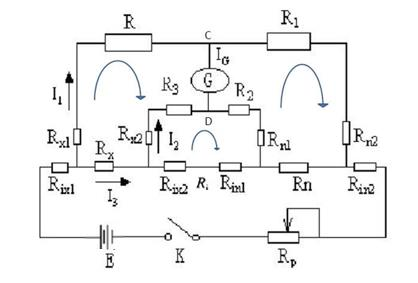
\includegraphics[width=0.7\textwidth]{circuit1.jpg}
    \caption{双臂电桥原理电路图}
\end{figure}

\begin{figure}[H]
    \centering
    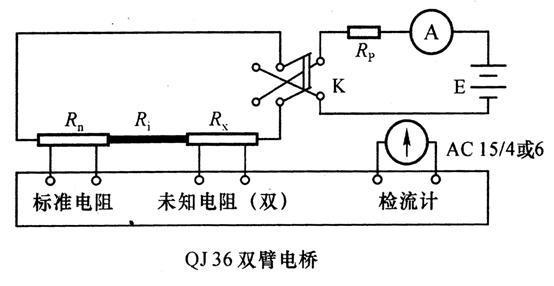
\includegraphics[width=0.7\textwidth]{circuit2.jpg}
    \caption{双臂电桥实验接线图}
\end{figure}

双臂电桥（凯尔文电桥）用于测量 $1\Omega$ 以下的低电阻，能有效消除接线电阻和接触电阻的影响。其原理电路如图 1 所示。
电路中 $R_x$ 为待测电阻，$R_n$ 为标准电阻，$r$ 为连接 $R_x$ 和 $R_n$ 的导线电阻。$R_1, R_2, R_3, R$ 为四个桥臂电阻。
当电桥平衡时，检流计 $G$ 中无电流流过，即 $C, D$ 两点电势相等。
根据基尔霍夫定律，可推导出电桥平衡条件为：
\[ R_x = \frac{R}{R_1} R_n + \frac{R R_i}{R_3 + R_2 + R_i} \left( \frac{R_2}{R_1} - \frac{R_3}{R} \right) \]
为了消除 $r$ 的影响，实验中调节桥臂电阻使 $\frac{R_2}{R_1} = \frac{R_3}{R}$ 始终成立。此时公式简化为：
\[ R_x = R_n \frac{R}{R_1} = 0.001 \times \frac{R}{1000} = R \times 10^{-6} \]
电阻率计算公式：
\[ \rho = \frac{R_x S}{L} = \frac{R_x \pi D^2}{4L} \]

\section{实验器材}
双臂电桥实验装置、标准电阻 $R_n$ ($0.001\Omega, 0.01$级)、电阻箱 ($R_1, R_2$等)、螺旋测微器、待测金属棒（铜、铝）、直流电源 ($U \approx 5V$)。

\section{原始数据}
\subsection{实验参数}
\begin{itemize}
    \item 螺旋测微器零误差：$d_0 = -0.006\,\text{mm}$
    \item 标准电阻：$R_n = 0.001\,\Omega$ (0.01级)
    \item 固定臂电阻：$R_1 = R_2 = 1000\,\Omega$
    \item 电源电压：$U = 4.9966\,\text{V}$
    \item 金属棒有效长度：$L = 30.00\,\text{cm} = 0.3000\,\text{m}$ (由分度值1mm直尺测定)
\end{itemize}

\subsection{测量数据表}

\begin{table}[H]
    \centering
    \caption{金属棒直径 $D$ 测量 (mm)}
    \begin{tabular}{cccccc}
        \toprule
        样品 & 1 & 2 & 3 & 平均值 $\bar{D}_{meas}$ & 修正后 $\bar{D}$ \\
        \midrule
        铜棒 & 4.951 & 4.956 & 4.959 & 4.9553 & 4.9613 \\
        铝棒 & 4.974 & 4.980 & 4.978 & 4.9773 & 4.9833 \\
        \bottomrule
    \end{tabular}

    \small{注：修正后值 $\bar{D} = \bar{D}_{meas} - d_0 = \bar{D}_{meas} + 0.006$}
\end{table}

\begin{table}[H]
    \centering
    \caption{平衡电阻箱读数 $R$ 测量 ($\Omega$)}
    \begin{tabular}{cccccccc}
        \toprule
        样品 & 方向 & 1 & 2 & 3 & 方向均值 & 总均值 $\bar{R}$ \\
        \midrule
        铜棒 & 正向 & 1205.00 & 1201.04 & 1199.34 & 1201.79 & \\
             & 反向 & 1211.00 & 1214.02 & 1215.20 & 1213.41 & 1207.60 \\
        \midrule
        铝棒 & 正向 & 554.42 & 551.20 & 551.53 & 552.38 & \\
             & 反向 & 556.60 & 557.37 & 556.20 & 556.72 & 554.55 \\
        \bottomrule
    \end{tabular}
\end{table}

\section{数据处理与不确定度计算}

\subsection{不确定度公式}
\begin{enumerate}
    \item \textbf{直径 $D$}：
    \[ u_A(D) = \sqrt{\frac{\sum(D_i - \bar{D})^2}{n(n-1)}}, \quad u_B(D) = \frac{\Delta_{inst}}{\sqrt{3}} = \frac{0.004}{\sqrt{3}} \approx 0.0023\,\text{mm} \]
    \[ u_c(D) = \sqrt{u_A^2 + u_B^2} \]
    \item \textbf{电阻箱读数 $R$}：
    电阻箱误差公式：$\Delta R = \pm(a\% R + nb)$，其中 $a=0.02, n=6, b=0.02$。
    \[ \Delta R = 0.0002 R + 0.12 \]
    \[ u_B(R) = \frac{\Delta R}{\sqrt{3}}, \quad u_A(R) = \sqrt{\frac{\sum(R_i - \bar{R})^2}{n(n-1)}} \]
    \[ u_c(R) = \sqrt{u_A^2 + u_B^2} \]
    \item \textbf{待测电阻 $R_x$}：
    由 $R_x = R_n \frac{R}{R_1}$，忽略 $R_1$ 误差，考虑 $R_n$ (0.01级) 和 $R$ 的误差：
    \[ \frac{u(R_x)}{R_x} = \sqrt{ \left(\frac{u(R_n)}{R_n}\right)^2 + \left(\frac{u_c(R)}{R}\right)^2 } \]
    其中 $u(R_n) = \frac{0.01\% R_n}{\sqrt{3}} = \frac{0.0001 \times 0.001}{\sqrt{3}}$。
    \item \textbf{电阻率 $\rho$}：
    \[ \frac{u(\rho)}{\rho} = \sqrt{ \left(\frac{u(R_x)}{R_x}\right)^2 + \left(2\frac{u_c(D)}{D}\right)^2 + \left(\frac{u(L)}{L}\right)^2 } \]
    其中 $u(L) = \frac{0.5}{\sqrt{3}} \approx 0.29\,\text{mm}$。
\end{enumerate}

\subsection{铜棒计算}
\begin{itemize}
    \item \textbf{直径}：$\bar{D} = 4.9613\,\text{mm}$。
    $u_A(D) = 0.0023\,\text{mm}$， $u_c(D) = \sqrt{0.0023^2 + 0.0023^2} = 0.0033\,\text{mm}$。
    \item \textbf{电阻读数}：$\bar{R} = 1207.60\,\Omega$。
    $u_A(R) \approx 2.71\,\Omega$ (根据6次数据)。
    $\Delta R = 0.0002 \times 1207.6 + 0.12 = 0.36\,\Omega$。
    $u_B(R) = 0.36 / \sqrt{3} = 0.21\,\Omega$。
    $u_c(R) = \sqrt{2.71^2 + 0.21^2} = 2.72\,\Omega$。
    \item \textbf{电阻 $R_x$}：
    \[ R_x = 1207.60 \times 10^{-6} = 1.2076 \times 10^{-3}\,\Omega = 1.2076\,\text{m}\Omega \]
    相对不确定度：
    $\frac{u(R_n)}{R_n} = \frac{0.0001}{\sqrt{3}} \approx 0.0058\%$。
    $\frac{u(R)}{R} = \frac{2.72}{1207.6} \approx 0.225\%$。
    合成后 $\frac{u(R_x)}{R_x} \approx 0.225\%$。
    $u(R_x) \approx 1.2076 \times 10^{-3} \times 0.00225 \approx 2.72 \times 10^{-6}\,\Omega$。
    \item \textbf{电阻率 $\rho$}：
    $S = \frac{\pi}{4}(4.9613\times 10^{-3})^2 = 1.9333 \times 10^{-5}\,\text{m}^2$。
    \[ \rho = \frac{1.2076 \times 10^{-3} \times 1.9333 \times 10^{-5}}{0.3000} = 7.782 \times 10^{-8}\,\Omega\cdot\text{m} \]
    相对不确定度：
    $u_{rel}(L) = \frac{0.29}{300} \approx 0.097\%$。
    \[ \frac{u(\rho)}{\rho} = \sqrt{(0.225\%)^2 + (2 \times \frac{0.0033}{4.9613})^2 + (0.097\%)^2} \approx 0.28\% \]
    $u(\rho) \approx 7.782 \times 10^{-8} \times 0.0028 \approx 0.022 \times 10^{-8}\,\Omega\cdot\text{m}$。
    结果：$\rho_{Cu} = (7.78 \pm 0.04) \times 10^{-8}\,\Omega\cdot\text{m}$ ($k=2$)。
\end{itemize}

\subsection{铝棒计算}
\begin{itemize}
    \item \textbf{直径}：$\bar{D} = 4.9833\,\text{mm}$。
    $u_A(D) = 0.0017\,\text{mm}$， $u_c(D) = \sqrt{0.0017^2 + 0.0023^2} = 0.0029\,\text{mm}$。
    \item \textbf{电阻读数}：$\bar{R} = 554.55\,\Omega$。
    $u_A(R) \approx 1.09\,\Omega$。
    $\Delta R = 0.0002 \times 554.55 + 0.12 = 0.23\,\Omega$。
    $u_B(R) = 0.23 / \sqrt{3} = 0.13\,\Omega$。
    $u_c(R) = \sqrt{1.09^2 + 0.13^2} = 1.10\,\Omega$。
    \item \textbf{电阻 $R_x$}：
    \[ R_x = 554.55 \times 10^{-6} = 5.5455 \times 10^{-4}\,\Omega = 0.5546\,\text{m}\Omega \]
    相对不确定度：$\frac{u(R)}{R} = \frac{1.10}{554.55} \approx 0.198\%$。
    $u(R_x) \approx 5.5455 \times 10^{-4} \times 0.00198 \approx 1.10 \times 10^{-6}\,\Omega$。
    \item \textbf{电阻率 $\rho$}：
    $S = \frac{\pi}{4}(4.9833\times 10^{-3})^2 = 1.9504 \times 10^{-5}\,\text{m}^2$。
    \[ \rho = \frac{5.5455 \times 10^{-4} \times 1.9504 \times 10^{-5}}{0.3000} = 3.605 \times 10^{-8}\,\Omega\cdot\text{m} \]
    相对不确定度：
    \[ \frac{u(\rho)}{\rho} = \sqrt{(0.198\%)^2 + (2 \times \frac{0.0029}{4.9833})^2 + (0.097\%)^2} \approx 0.25\% \]
    $u(\rho) \approx 3.605 \times 10^{-8} \times 0.0025 \approx 0.009 \times 10^{-8}\,\Omega\cdot\text{m}$。
    结果：$\rho_{Al} = (3.61 \pm 0.02) \times 10^{-8}\,\Omega\cdot\text{m}$ ($k=2$)。
\end{itemize}

\section{结论与讨论}
\begin{enumerate}
    \item 铜棒电阻率测得值为 $\rho_{Cu} = (7.78 \pm 0.04) \times 10^{-8}\,\Omega\cdot\text{m}$ ($k=2$)。
    \item 铝棒电阻率测得值为 $\rho_{Al} = (3.61 \pm 0.02) \times 10^{-8}\,\Omega\cdot\text{m}$ ($k=2$)。
    \item 注：结果中的不确定度为扩展不确定度 $U = k \cdot u_c$，其中 $k=2$ 为包含因子，对应约 95\% 的置信概率。
    \item 讨论：
    \begin{itemize}
        \item 铝棒的测量值 ($3.61 \times 10^{-8}$) 与标准值 ($2.7 \times 10^{-8}$) 较为接近，考虑到实验误差和材料纯度，结果较为合理。
        \item 铜棒的测量值 ($7.78 \times 10^{-8}$) 显著高于纯铜的标准值 ($1.7 \times 10^{-8}$)。这可能是因为该“铜棒”实际上是黄铜（电阻率约 $6 \sim 7 \times 10^{-8}\,\Omega\cdot\text{m}$）或其他铜合金，而非纯铜。
    \end{itemize}
\end{enumerate}

\section{原始数据记录}
\begin{figure}[H]
    \centering
    
\includegraphics[width=0.7\textwidth]{原始数据.jpg}
    \caption{老师签字的原始数据}
\end{figure}

\end{document}
